\documentclass[a4paper, 12pt]{article}

\usepackage[utf8]{inputenc}
\usepackage[russian]{babel}
\usepackage{graphicx}
\graphicspath{{pictures/}}
\DeclareGraphicsExtensions{.pdf,.png,.jpg, .jpeg}
\usepackage[unicode, pdftex]{hyperref}
\usepackage{color}
\usepackage{float}
\setlength{\parindent}{5ex}
\setlength{\parskip}{1em}
\usepackage{indentfirst}
\addto\captionsrussian{\def\refname{Список используемых источников}}

\begin{document}

\begin{titlepage}
  \thispagestyle{empty}
  \centerline {Санкт-Петербургский политехнический университет}
  \centerline { им. Петра Великого}
  \centerline { }
  \centerline {Институт прикладной математики и механики} 
  \centerline {Кафедра "Прикладная математика"}
  \vfill
  \centerline{\textbf{Курсовая работа}}
  \centerline{\textbf{по дисциплине}}
  \centerline{\textbf{"Математическая статистика"}}
  \centerline{ }
  \centerline{\textbf{Разведочный анализ данных}}
  \vfill
  \hfill
  \begin{minipage}{0.45\textwidth}
  Выполнила студентка:\\
  Дроздова Дарья Александровна \\
  группа: 3630102/80401 \\
  \\
  Проверил:\\
  к.ф.-м.н., доцент \\
  Баженов Александр Николаевич
  \end{minipage}
  \vfill
  \centerline {Санкт-Петербург}   
  \centerline {2021 г.}  
\end{titlepage}

\newpage
\setcounter{page}{2}
\tableofcontents

\newpage
\listoffigures

\newpage
\section*{Введение}
\addcontentsline{toc}{section}{Введение}

Разведочый анализ данных (РАД) - предварительное исследование набора данных с целью  определения его основных характеристик, взаимосвязей между признаками. РАД употребляется, когда с одной стороны, у исследователя имеется таблица многомерных данных, а с другой стороны, априорная информация о физическом (причинном) механизме генерации этих данных отсутствует или неполна.

\newpage
\section*{Основная часть}
\addcontentsline{toc}{section}{Основная часть}

\section{Определение разведочного анализа}

\subsection{Цель разведочного анализа}

Если априорная информация о предмете исследования отсутствует, тогда разведочный анализ помогает исследователю в компактном и понятном описании структуры данных, например, в форме визуального представления данной структуры, отталкиваясь от которого можно поставить наиболее точный вопрос исследования данных с помощью того или иного раздела статистического анализа, а также сделать вывод о причинной модели данных и т. д. Этот этап называется "подтверждающим анализом". Иногда выявление структуры данных с помощью РАД может оказаться завершающим этапом анализа. С другой стороны, методы РАД можно рассматривать и как методы подготовки данных для последующей статистической обработки без какого-либо изучения структуры данных, которое предлагается осуществить на последующих этапах. В этом случае этап РАД играет роль некоторого этапа перекодировки и преобразования данных, например, сокращение размерности, в удобную для последующего анализа форму. 

С какой бы целью ни применялись методы РАД, основная задача: переход к компактному описанию данных при возможно более полном сохранении существенных аспектов информации, содержащихся в исходных данных.

Впервые термин "разведочный анализ данных" был введен Дж. Тьюки в 1962 г.

\subsection{Модели структуры многомерных данных в разведочном анализе}

Пусть данные заданы в виде матрицы данных. Объекты можно представить в виде точек в многомерном пространстве. Для описания структуры этого множества в РАД используется одна из следующих статистических моделей:
\begin{itemize}
	\item модель облака точек примерно эллипсоидальной конфигурации
	\item кластерная модель, т. е. совокупность нескольких "облаков" точек, достаточно далеко отстоящих друг от друга
	\item модель "засорения", т. е. компактное облако точек и при этом присутствуют далекие выбросы
	\item модель носителя точек как многообразия (линейного или нелинейного) более низкой размерности, чем исходное (например, выборка из вырожденного распределения)
	\item дискриминантная модель, когда точки разделены некоторым образом на несколько групп и дана информация о их принадлежность к той или иной группе.
\end{itemize}

\subsection{Модели описания структуры зависимостей в разведочном анализе}

В пространстве переменных для описания структуры зависимостей между переменными часто используются следующие модели:
\begin{itemize}
	\item Модель независимых переменных
	\item Модель линейно зависимых переменных
	\item Древообразная модель зависимости
	\item Факторная модель для линейно зависимых переменных
	\item Кластерная модель 
	\item Иерархическая модель зависимости
\end{itemize}

\subsection{Основные приемы проведения разведочного анализа}

Способы анализа и интерпретации результатов в значительной степени зависят от выбранного метода обработки. Однако можно выделить ряд эффективных приемов и подходов к анализу результатов, которые являются наиболее общими и в значительной степени определяют специфику разведочного анализа, к ним относятся:
\begin{itemize}
	\item Визуализация данных
	\item Манипуляции с данными на основе графического отображения
	\item Использования аппарата активных и иллюстративных переменных 
	\item Преобразование данных
	\item Анализ остатков
\end{itemize}



\section{Визуализация данных}

\subsection{Роль визуализации данных в разведочном анализе}

Основная функция РАД - дать компактное и понятное описание структур данных или структуры зависимости переменных. Визуализация данных, которая предполагает получение тем или иным способом их графического отображения, так что исследователь может путем визуального анализа определить имеет ли место одна из моделей структуры данных, является наиболее наглядным способом описания. 

Графическое отображение (гистограммы, диаграммы рассеивания) может быть получено непосредственно в пространстве исходных переменных. Однако, информативное графическое отображение многомерных данных получается с помощью методов РАД, нацеленных на выявление перечисленных структур данных и зависимостей. В результате применения этих методов получаются образы объектов, переменных и для не количественных переменных категория в виде точек (обычно размерности 1-3). Выходная размерность данных может быть и больше 3, но для графического отображения все равно берутся какие-либо 1-3 координаты, обычно при этом первые координаты более информативны и используются для визуального анализа в первую очередь. 

\subsection{Гистограмма}

Гистограмма визуализирует распределение данных в рамках непрерывного интервала или ограниченного периода времени. Каждая полоса на гистограмме представляет в табличной форме частотность за определенный интервал. Общая площадь гистограммы равна количеству данных.

Гистограммы помогают определить концентрацию значений, предельные значения и наличие пробелов или отклонений. Кроме того, они удобны для составления приблизительного обзора распределения вероятностей.

\begin{figure}[H]
\center{\includegraphics[scale=0.4]{gist}}
\caption{Пример гистограммы}
\end{figure}

\subsection{Диаграммы рассеивания}

Диаграмма рассеивания многомерных данных является визуальной формой представления результатов некоторого отображения исходной матрицы данных в двумерное евклидово пространство. Роль исходной матрицы может играть матрица "объект-свойство" или матрица близостей (отношений "объект-объект", "переменная-переменная"). В качестве отображенных на диаграмме рассеивания единиц могут выступать объекты, переменные, категории переменных (если переменные не количественные). 

\begin{figure}[H]
\center{\includegraphics[scale=0.4]{dr}}
\caption{Пример диаграммы рассеивания}
\end{figure}

\section{Преобразование данных  в разведочном анализе данных}

Пусть исходные данные даны в виде матрицы "объект-признак". Нелинейные преобразования в РАД могут быть использованы для линеаризации зависимостей между переменными, для упрощения структуры данных

\subsection{Линеаризация зависимостей между переменными}

Цель таких преобразований состоит в переходе к новому набору переменных, зависимость между которыми является более близкой к линейной. Если такое преобразование удается найти, то дальше к новой матрице данных можно применять линейные статистические методы: главные компоненты, факторный анализ, линейная регрессия и т. д.

\subsection{Упрощение структуры данных}

В этом случае стремятся получить преобразования, после применения которых распределение становится максимально похожим на многомерное нормальное. 

\section{Использование дополнительных переменных и объектов}

При использовании методов РАД существует опасность обнаружить в данных такие структуры, которые связаны, скорее, со спецификой данной выборки, но в силу ее недостаточного объема не отражают каких-либо устойчивых закономерностей в генеральной совокупности. В случае, когда исследуемое множество объектов само представляет собой всю генеральную совокупность, такой проблемы не возникает, однако, если результаты, полученные при изучении выборки, будут использоваться для работы с объектами, не входящими в нее, тогда могут возникнуть проблемы.

Существует прием для решения этой проблемы, который состоит в разделении объектов и переменных на две части - активные (объекты и переменные) и иллюстративные, экзаменующие. Разделение объектов на "обучение" и "экзамен" широко используется в дискриминантном и регрессионным анализе. 

Помимо проверки устойчивости выделенных структур, использование дополнительных элементов помогает и в интерпретации РАД.

\section{Основные типы данных и методы, используемые в разведочном анализе данных}

РАД применяется к данным, заданным в одной из следующих форм:
\begin{enumerate}
	\item матрица данных типа "объект-признак" с переменными, измеренными в количественных шкалах
	\item матрица данных с переменными, измеренными в ординальной шкале
	\item матрица данных с переменными, измеренными в номинальной шкале
	\item матрица данных с переменными, измеренными в шкалах разной природы
	\item таблица данных типа "объект-объект"
	\item таблица сопряженностей
\end{enumerate}

Процедуры статистической обработки, используемые в РАД, могут быть разбиты на следующие группы в зависимости от целей анализа и типа обрабатываемых данных:
\begin{itemize}
	\item Вычисление основных статистических характеристик для матрицы типа 1
	\item Преобразование переменных для матриц типа 1 с целью линеаризации связей и нормализации данных симметризации
	\item Преобразование переменных для матриц типа 1, 2, 3, 4
	\item Сокращение размерности данных с помощью линейных отображений: главные компоненты, целенаправленное проецирование
	\item Нелинейные методы отображения данных для матриц типа 1, 2, 3, 4
	\item Метрическое шкалирование для матриц типа 5
	\item Множественный анализ соответствий для матриц типа 2, 3, 4, 6
	\item Классификационные методы: кластер-анализ для таблиц для матриц типа 1, 2, 3, 5, разделение смесей распределений, дискриминантный анализ
	\item Топологический анализ главных компонент. Анализ древообразной структуры зависимостей для матрицы типа 1
	\item Кластер-анализ переменных матриц типа 1, 2, 3, 4, 6. Пошаговый метод анализа структуры зависимостей переменных для матриц типа 2, 3, 6
	\item Анализ регрессионных зависимостей
\end{itemize}

\section{Разведочный анализ данных DRS}

На основании данных для DRS построены гистограммы распределения ширин ячеек.

Ссылка на данные находится в Приложении 1.

\begin{figure}[H]
\center{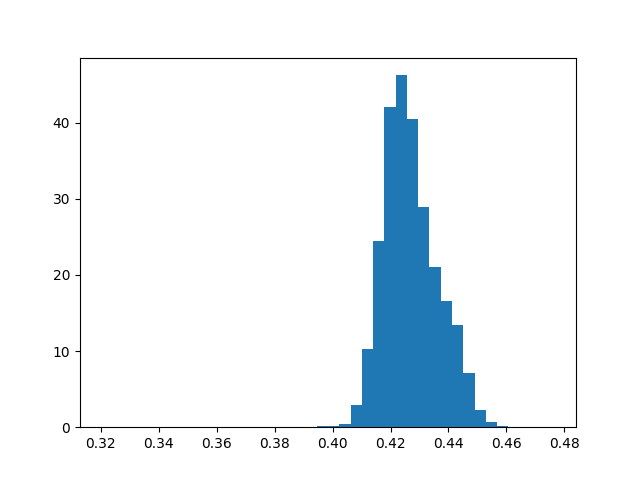
\includegraphics[scale=0.4]{+0_5V}}
\caption{Гистограмма распределения ширин ячеек для +0,5V}
\end{figure}

\begin{figure}[H]
\center{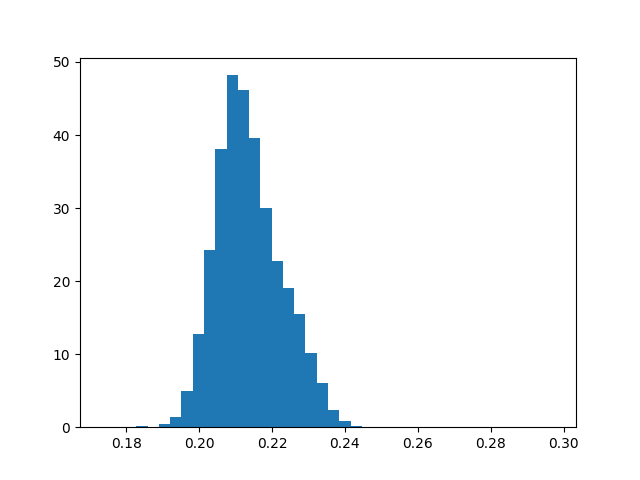
\includegraphics[scale=0.4]{+0_25V}}
\caption{Гистограмма распределения ширин ячеек для +0,25V}
\end{figure}

\begin{figure}[H]
\center{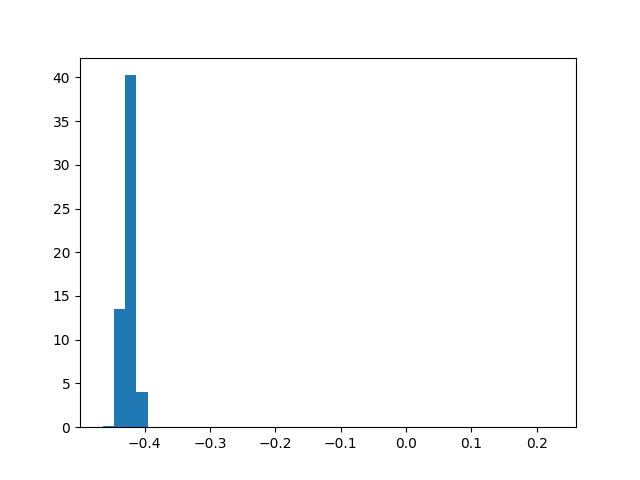
\includegraphics[scale=0.4]{-0_5V}}
\caption{Гистограмма распределения ширин ячеек для -0,5V}
\end{figure}

\begin{figure}[H]
\center{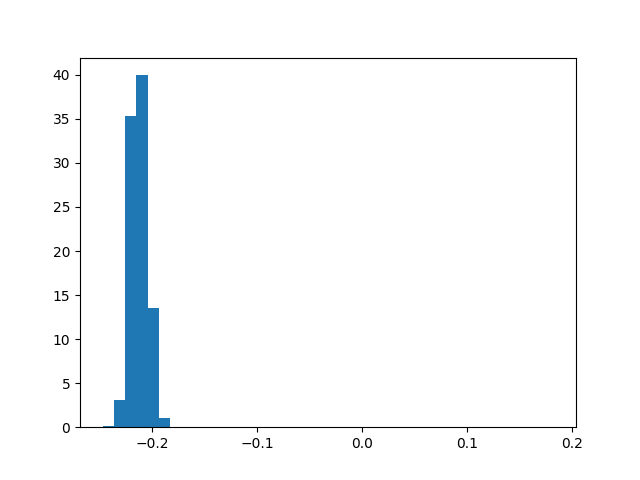
\includegraphics[scale=0.4]{-0_25V}}
\caption{Гистограмма распределения ширин ячеек для -0,25V}
\end{figure}

\begin{figure}[H]
\center{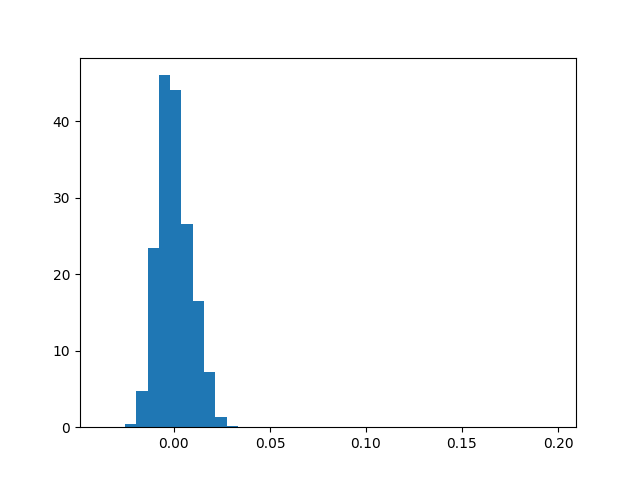
\includegraphics[scale=0.4]{ZeroLine}}
\caption{Гистограмма распределения ширин ячеек для нулевой линии}
\end{figure}

\begin{figure}[H]
\center{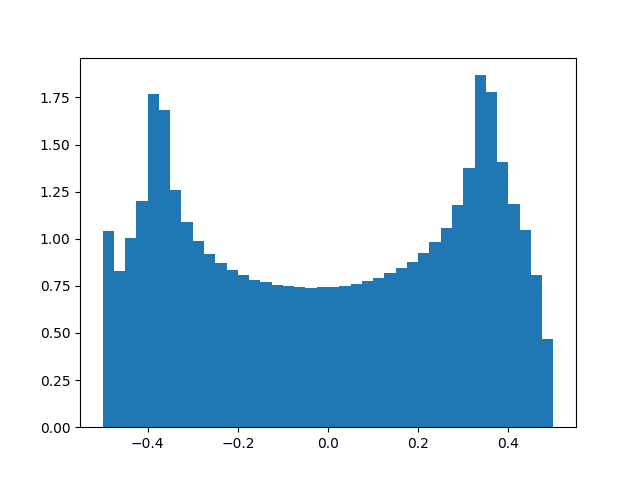
\includegraphics[scale=0.4]{Sin_100MHz}}
\caption{Гистограмма распределения ширин ячеек для набора синусоид}
\end{figure}

\newpage
\section*{Заключение}
\addcontentsline{toc}{section}{Заключение}

Этап РАД применяется, когда у исследователя отсутствует априорная информация о статистическом или причинном механизме порождения имеющихся в его распоряжении данных. Основная цель РАД - построить некоторую статистическую модель данных. Можно сказать, что на этапе РАД формулируются статистическое гипотезы, которые должны быть проверены на этапе подтверждающего анализа.

Важнейшим элементом РАД является широкое использование визуального представления многомерных данных, возможности которого возросли с появлением динамических форм визуального представления

Преобразование данных в РАД позволяет или линеаризировать связи между переменными, или упростить для дальнейшего описания структуры данных.

Для верификации результатов РАД эффективном примером может являться использование аппарата иллюстративных переменных и объектов.

\newpage
\addcontentsline{toc}{section}{Список используемых источников}
\begin{thebibliography}{}
    \bibitem{litlink1} Дж. Тьюки. Анализ результатов наблюдений. Разведочный анализ. М.: Мир, 1981. Пер. изд.: John W. Tukey. Exploratory Data Analysis. Massachusetts: Addison-Wesley Publishing Company Reading, 1977.
    \bibitem{litlink2} Андерсон К. Аналитическая культура. От сбора данных до бизнес-результатов / К. Андерсон - "Манн, Иванов и Фербер", 2015
    \bibitem{litlink3} Paul Scherrer Institut. 9 Channel, 5 GSPS Switched Capacitor Array, DRS4 
    
\end{thebibliography}

\newpage
\section*{Приложение 1} \label{pr}
\addcontentsline{toc}{section}{Приложение 1}

Код программы и данные расположены в репозитории GitHub по ссылке: \url{https://github.com/Drozdova-Daria/Math_Stat_KR}
\end{document}
